%% This Beamer template is based on the one found here: https://github.com/sanhacheong/stanford-beamer-presentation, and edited to be used for Stanford ARM Lab

\documentclass[10pt]{beamer}
%\mode<presentation>{}

\usepackage{media9}
\usepackage{amssymb,amsmath,amsthm,enumerate}
\usepackage[utf8]{inputenc}
\usepackage{array}
\usepackage[parfill]{parskip}
\usepackage{graphicx}
\usepackage{caption}
\usepackage{subcaption}
\usepackage{bm}
\usepackage{amsfonts,amscd}
\usepackage[]{units}
\usepackage{listings}
\usepackage{multicol}
\usepackage{multirow}
\usepackage{tcolorbox}
\usepackage{physics}
%encoding
%--------------------------------------
\usepackage[T1]{fontenc}
\usepackage[utf8]{inputenc}
%--------------------------------------

%Portuguese-specific commands
%--------------------------------------
\usepackage[portuguese]{babel}
%--------------------------------------

%Hyphenation rules
%--------------------------------------
\usepackage{hyphenat}
\hyphenation{mate-mática recu-perar}
%--------------------------------------

% Enable colored hyperlinks
\hypersetup{colorlinks=true}

% The following three lines are for crossmarks & checkmarks
\usepackage{pifont}% http://ctan.org/pkg/pifont
\newcommand{\cmark}{\ding{51}}%
\newcommand{\xmark}{\ding{55}}%

% Numbered captions of tables, pictures, etc.
\setbeamertemplate{caption}[numbered]

%\usepackage[superscript,biblabel]{cite}
\usepackage{algorithm2e}
\renewcommand{\thealgocf}{}

% Bibliography settings
\usepackage[style=ieee]{biblatex}
\setbeamertemplate{bibliography item}{\insertbiblabel}
\addbibresource{references.bib}

% Glossary entries
\usepackage[acronym]{glossaries}
\newacronym{ML}{ML}{machine learning}
\newacronym{HRI}{HRI}{human-robot interactions}
\newacronym{RNN}{RNN}{Recurrent Neural Network}
\newacronym{LSTM}{LSTM}{Long Short-Term Memory}


\theoremstyle{remark}
\newtheorem*{remark}{Remark}
\theoremstyle{definition}

\newcommand{\empy}[1]{{\color{darkorange}\emph{#1}}}
\newcommand{\empr}[1]{{\color{cardinalred}\emph{#1}}}
\newcommand{\examplebox}[2]{
\begin{tcolorbox}[colframe=darkcardinal,colback=boxgray,title=#1]
#2
\end{tcolorbox}}

\usetheme{Stanford} 
\def \i  {\item}
\def \ai {\item[] \quad \arrowbullet}
\newcommand \si[1]{\item[] \quad \bulletcolor{#1}}
\def \wi {\item[] \quad $\ \phantom{\Rightarrow}\ $}
\def \bi {\begin{itemize}\item}
\def \ei {\end{itemize}}
\def \be {\begin{equation*}}
\def \ee {\end{equation*}}
\def \bie {$\displaystyle{}
\def \eie {{\ }$}}
\def \bsie {\small$\displaystyle{}
\def \esie {{\ }$}\normalsize\selectfont}
\def \bse {\small\begin{equation*}}
\def \ese {\end{equation*}\normalsize}
\def \bfe {\footnotesize\begin{equation*}}
\def \efe {\end{equation*}\normalsize}
\renewcommand \le[1] {\\ \medskip \lefteqn{\hspace{1cm}#1} \medskip}
\def \bex {\begin{example}}
\def \eex {\end{example}}
\def \bfig {\begin{figure}}
\def \efig {\end{figure}}
\def \btheo {\begin{theorem}}
\def \etheo {\end{theorem}}
\def \bc {\begin{columns}}
\def \ec {\end{columns}}
\def \btab {\begin{tabbing}}
\def \etab {\end{tabbing}\svneg\svneg}
\newcommand \col[1]{\column{#1\linewidth}}
\def\vneg  {\vspace{-5mm}}
\def\lvneg {\vspace{-10mm}}
\def\svneg {\vspace{-2mm}}
\def\tvneg {\vspace{-1mm}}
\def\vpos  {\vspace{5mm}}
\def\lvpos {\vspace{10mm}}
\def\svpos {\vspace{2mm}}
\def\tvpos {\vspace{1mm}}
\def\hneg  {\hspace{-5mm}}
\def\lhneg {\hspace{-10mm}}
\def\shneg {\hspace{-2mm}}
\def\thneg {\hspace{-1mm}}
\def\hpos  {\hspace{5mm}}
\def\lhpos {\hspace{10mm}}
\def\shpos {\hspace{2mm}}

\logo{
\includegraphics[height=0.4in]{./images/logoufjf10.png}}

% commands to relax beamer and subfig conflicts
% see here: https://tex.stackexchange.com/questions/426088/texlive-pretest-2018-beamer-and-subfig-collide
\makeatletter
\let\@@magyar@captionfix\relax
\makeatother

\newcommand{\code}[1]{\textcolor{red} {\textit{#1}}} %comentarios

\title[Reunião de Orientação 04]{Reunião de Orientação 04}
%\subtitle{Subtitle Of Presentation}

%\beamertemplatenavigationsymbolsempty

\begin{document}

\author[Modelagem Computacional]{
	\begin{tabular}{c} 
	\Large
	Igor Pires dos Santos\\
    \footnotesize \href{mailto:igor.pires@ice.ufjf.br}{igor.pires@ice.ufjf.br}\\
    \textbf{Orientador:} Rafael Bonfim
\end{tabular}
\vspace{-4ex}}

\institute{
	\vskip 5pt
	\begin{figure}
		\centering
		\begin{subfigure}[t]{0.5\textwidth}
			\centering
			
\includegraphics[height=0.33in]{images/logoufjf1}
		\end{subfigure}%
		~ 
		\begin{subfigure}[t]{0.5\textwidth}
			\centering
			
\includegraphics[height=0.33in]{./images/PGMC.png}
		\end{subfigure}
	\end{figure}
	\vskip 5pt
	Programa de Pós-Graduação em Modelagem Computacional\\
	Universidade Federal de Juiz de Fora\\
	\vskip 3pt
}

% \date{June 15, 2020}
\date{\today}

\begin{noheadline}
\begin{frame}\maketitle\end{frame}
\end{noheadline}

\setbeamertemplate{itemize items}[default]
\setbeamertemplate{itemize subitem}[circle]

\begin{frame}
	\frametitle{Sumário} % Table of contents slide, comment this block out to remove it
	\tableofcontents % Throughout your presentation, if you choose to use \section{} and \subsection{} commands, these will automatically be printed on this slide as an overview of your presentation
\end{frame}

\section{Introdução}
\begin{frame}[allowframebreaks]
\frametitle{Avanços}
	
	\begin{itemize}
		\item \textbf{Proposta Passada}
		\item Outubro: Realização do Toefl iBT, Adicionar possibilidade de se executar o IGU 1.0 via linha de comando, Finalizar Repositório de imagem com o IGU 1.0 Instalado, Definir os experimentos relevantes com CCO (Ye, Pressão e Fluxo?)(Quais parâmetros ?), Definir se um sistema de CI/CD será aplicado e QUAL e COMO.
		
		\item Novembro: Finalização da Graduação, Rodar os experimentos relevantes com CCO utilizando o IGU 1.0 , escrever (e plotar) estes resultados.
		
		\item Dezembro: Finalizar parte Gráfica IGU 2.0, finalizar sistema de CI/CD, re-analisar funcionalidades do IGU 2.0 à adicionar e começar dissertação.
		
		\item Janeiro: Começar IGU 2.0 e sua parte distribuída e escrever dissertação.
		
	\end{itemize}
	
	
	\framebreak
	
	\begin{itemize}
		\item \textbf{Proposta Atualizada}
		\item Outubro: Realização do Toefl iBT, \red{Adicionar possibilidade de se executar o IGU via linha de comando (InGU), Definir os experimentos relevantes com CCO}
		
		\item Novembro:  \red{Finalização da Graduação}, \yellow{Rodar os experimentos relevantes com CCO utilizando o IGU } , escrever (e plotar) estes resultados.
		
		\item Dezembro: Finalizar parte Gráfica IGU atualizada, finalizar sistema de CI/CD, re-analisar funcionalidades do IGU à adicionar e começar dissertação.
		
		\item Janeiro: Começar parte distribuída e escrever dissertação.
		
	\end{itemize}
	
	
	\framebreak
	
	\begin{itemize}
		\item \textbf{O ciclo de vida de um software}
		
	\end{itemize}
	
	\begin{center}
		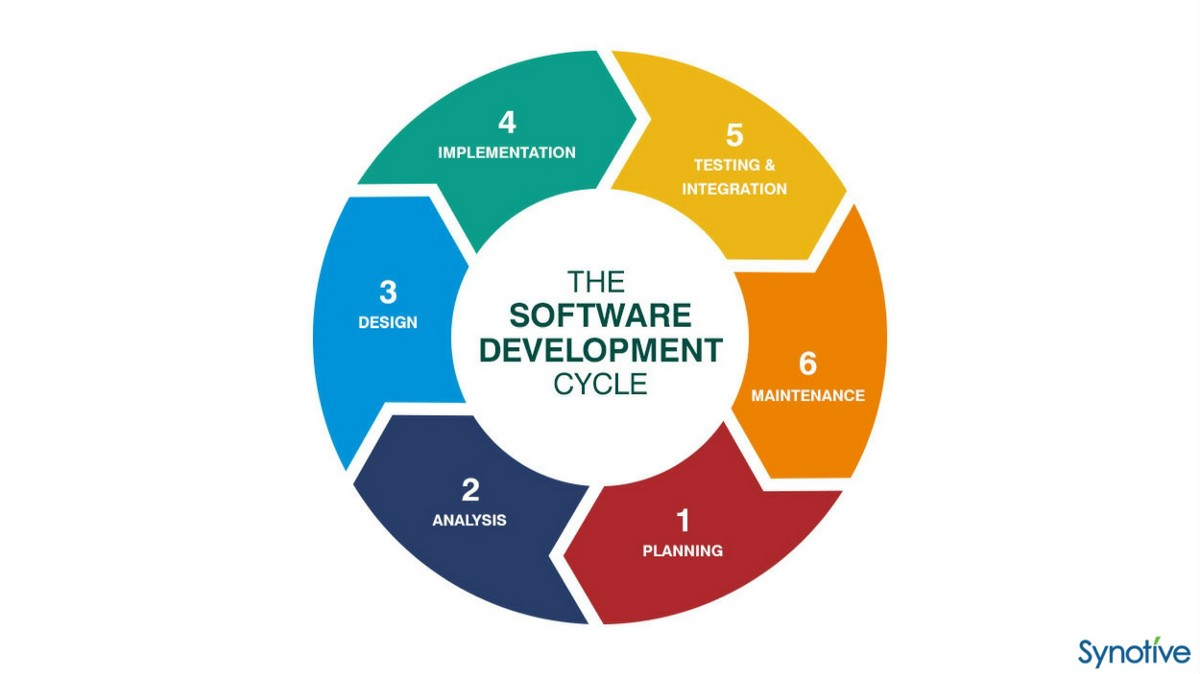
\includegraphics[width=0.7\textwidth]{images/05.jpg}
	\end{center}
	
	
	\framebreak
	
	\begin{itemize}
	
		\item Pensando na situação atual em que possua o código do IGU e em paralelo possuo esse código do "IGU 2.0", toda modificação que eu faria no código anterior se torna antiquada, porque na primeira versão as conexões entre os objetos (gráficos & árvores arterias, basicamente os objetos inteligentes) eram estáticas.
		
		\item Ainda na primeira versão todos os objetos eram também obrigatoriamente gráficos. Enfim, diversas mudanças novas no código acarretariam em soluções antiquadas no novo contexto do IGU 2.0 que apresentaria uma solução mais simples e unificada. Possibilitando ainda a parametrização de todas as variáveis (uma vez que o arquivo VTK é lido e pode ser manipulado, escalado e itera), podendo ainda ter ou não o fator gráfico e ainda trocar o método iterativo em tempo de execução.
		
	\end{itemize}
	
	
	\framebreak
	
	\begin{itemize}
		\item Pensando nisso e nas atividades conseguintes eu juntei os dois projetos de forma separada, dentro do mesmo repositório agora possuirei 3 compiláveis (nomes sugestivos):
		
		\item IGU: Iterador Gráfico Universal, IGU "antigo" com todo o seu código e parte gráfica.
		
		\item InGU: Iterador não-Gráfico Universal, programa console com toda a arquitetura IGU atualizada.
		
		\item PERIGU: PERimeter for IGU: Programa console simples que alterna entre as versões do programa (opcional, simplifica na hora de executar comandos do console).
		
	\end{itemize}
	
	
	\framebreak
	
	\begin{itemize}
		\item InGU + IGU
		
		\item (mostrar no Qt)
	\end{itemize}
	
\end{frame}

\end{document}